\documentclass{standalone}
\usepackage{tikz}

\begin{document}

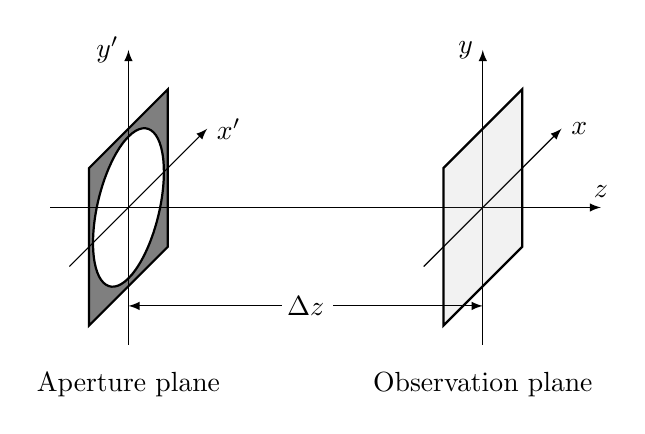
\begin{tikzpicture}[z={(1cm,0cm)},x={(0.5cm,0.5cm)}, y={(0cm,1cm)}, scale=1]

    % constants
    \def\zimg{4.5}
    
    % coordinate system 
    \coordinate (0) at (0,0,0);
    \draw[-latex] (0) -- +(2,0,0) node [right] {$x'$};
    \draw (0) -- +(-1.5,0,0);
    \draw[-latex] (0) -- +(0,2,0) node [left] {$y'$};
    \draw (0) -- +(0,-1.75,0);
    \draw[-latex] (0) -- +(0,0,6) node [above] {$z$};
    \draw (0) -- +(0,0,-1);
    
    \coordinate (2) at (0,0,\zimg);
    \draw[-latex] (2) -- +(2,0,0) node [right] {$x$};
    \draw (2) -- +(-1.5,0,0);
    \draw[-latex] (2) -- +(0,2,0) node [left] {$y$};
    \draw (2) -- +(0,-1.75,0);

    % Aperture plane
    \draw [thick, fill=black, fill opacity=0.5, even odd rule] 
        (-1,-1,0) -- (1,-1,0) -- (1,1,0) -- (-1,1,0) -- cycle (0,0) 
        circle[radius=0.9]; 
    \node [align=left] at (0,-2.25,0) {Aperture plane};
    %\draw[-latex] (-1.5,-0.75,0) -- (-0.25,-0.5,0);
    %\node [left] at (-1.3,-0.9,0) {$\mathbf{A}$};

    % Observation plane 
    \draw [thick,fill=gray,fill opacity=0.1] (-1,-1,\zimg) -- (1,-1,\zimg) -- (1,1,\zimg) -- (-1,1,\zimg) -- cycle; 
    \node [align=center] at (0,-2.25,\zimg) {Observation plane};

    % Ray
    \draw [latex-] (0,-1.25,0) -- (0,-1.25,1.95);
    \draw [-latex] (0,-1.25,2.6) -- (0,-1.25,\zimg);
    \node [align=center] at (0,-1.25,2.25) {$\Delta z$};

\end{tikzpicture}

\end{document}
